\begin{figure}[htbp]
\centering
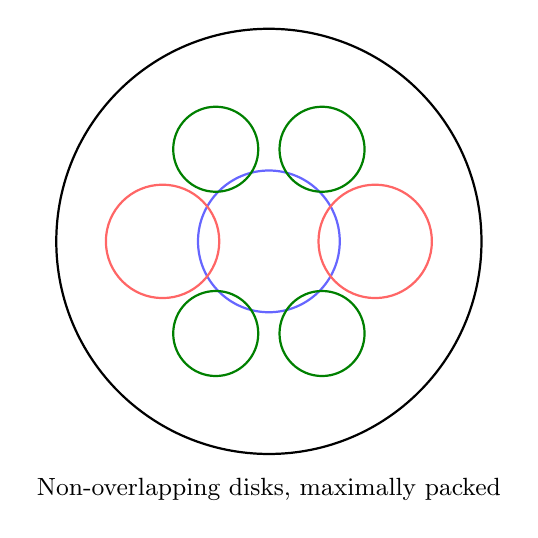
\begin{tikzpicture}[scale=0.9]
  \draw[thick] (0,0) circle (3);
  \draw[blue!60,thick] (0,0) circle (1);
  \draw[red!60,thick] (1.5,0) circle (0.8);
  \draw[red!60,thick] (-1.5,0) circle (0.8);
  \draw[green!50!black,thick] (0.75,1.3) circle (0.6);
  \draw[green!50!black,thick] (-0.75,1.3) circle (0.6);
  \draw[green!50!black,thick] (0.75,-1.3) circle (0.6);
  \draw[green!50!black,thick] (-0.75,-1.3) circle (0.6);
  \node[font=\small] at (0,-3.5) {Non-overlapping disks, maximally packed};
\end{tikzpicture}
\caption{Circle packing: placing non-overlapping disks of varying radii inside a bounding region.}
\label{fig:circle_packing}
\end{figure}
